%!TEX root = ../Thesis.tex
\chapter{Plan}


\section{Gantt Chart}

\noindent
Figure~\ref{fig:gantt} shows an outline of the project plan, which extends 18 weeks (Feb 2nd - June 7th, 2026), including the studying, creation, and documentation of the pipeline in question.

\begin{figure}[htbp]
    \centering
    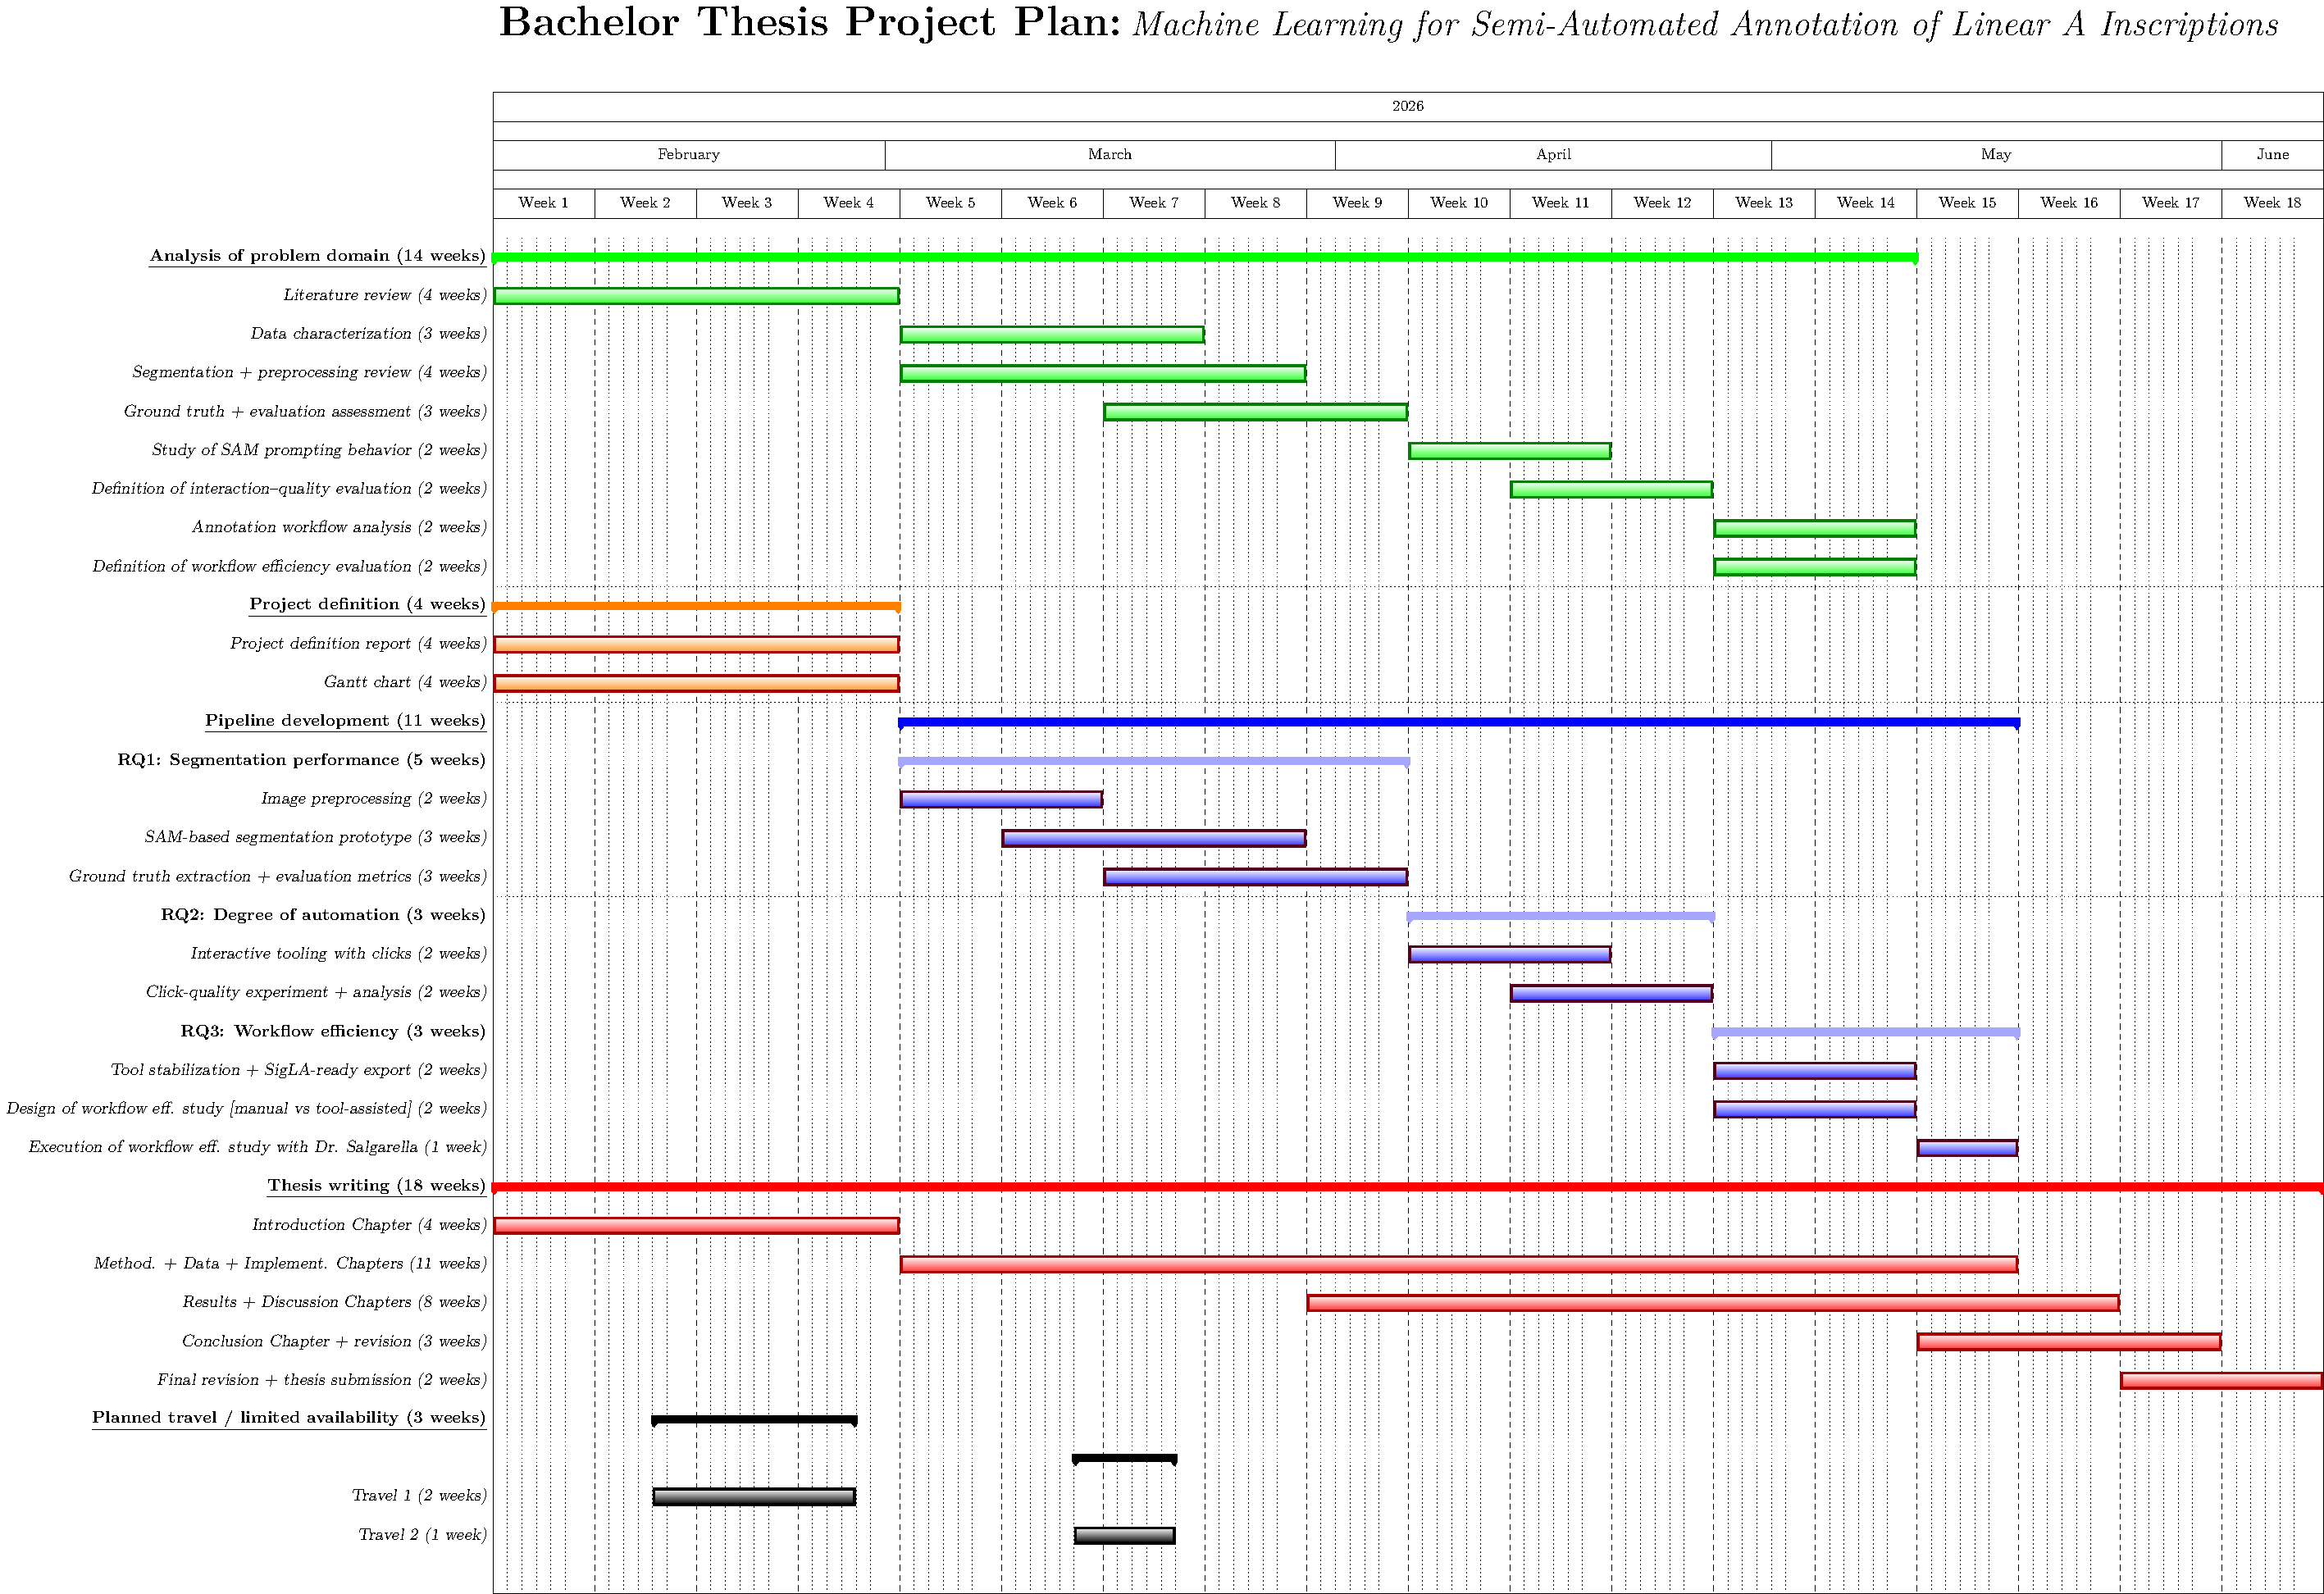
\includegraphics[width=\textwidth]{gantt/gantt.pdf}
    \caption{Project timeline (Gantt chart). See the appendix for a larger version (Fig.~\ref{fig:gantt_appendix})}
    \label{fig:gantt}
\end{figure}

\noindent
This chart is divided into five groups of work packages, all complementing each other. These are (from top to bottom): 
\begin{itemize}
    \item in green, \textit{Analysis of problem domain}: the study of the relevant literature and analysis required to proceed with the pipeline development. Work packages belonging to this group are placed in parallel with development, as they are necessary to inform it.
    \item in orange, \textit{Project definition}: the writing up of this \acf{PDR} including its project plan and Gantt chart.
    \item in blue, \textit{Pipeline development}: the creation of the segmentation tool pipeline to be delivered. In work package subgroups, this is split up by relevance to the three research questions, whose answers will continously compliment each other, as the work is carried out. These are:
    \begin{itemize}
        \item \textit{RQ1 (Segmentation Performance)}: the development and evaluation of the tool's initial segmentation performance. This is necessary to proceed with the next steps, as no comparison or extended version of the tool can be built without it.
        \item \textit{RQ2 (Degree of Automation)}: the development of tool interactivity and evaluation of its degree of automation. This is necessary to proceed with the final step, as the tool needs to be in its full interactive form before it can be tested in a real-world setting.
        \item \textit{RQ3 (Workflow Efficiency)}: the stabilization and final evaluation of the tool's workflow efficiency. This is where all the previous work comes together to answer the question of the tool's practical value and ability to contribute to the digitization workflow of SigLA.
    \end{itemize}
    \item in red, \textit{Thesis writing}: the simultaneous writing up of the thesis, including its chapters, revision and submission. The method, data and implementation chapters will be written together in parallel with pipeline development, while the results and discussion chapters will be mostly written during evaluation work, which is carried out at the end of each research question's development phase.
    \item in black, \textit{Planned travel / limited availability}: the periods where the author will have limited availability due to travel. These are included, as they might affect the project timeline, and have been taken into account in the planning of the work packages.
\end{itemize}
The in-group work packages partly overlapping in time, signals that they might have to be carried out in parallel during the transitions between them. 


\section{Milestones}
Although each work package functions as its own milestone, deliverable and deadline, there are a few key milestones in the project that are especially important to keep track of.
These are summarized in Table~\ref{tab:milestones}.

\begin{table}[h]
\caption{Milestones. D: Deadline, B: Buffer, TH: Thesis}
\centering{
\scriptsize{
\begin{tabular}{|c p{2.0cm}| p{5.0cm}| c | c|}
\toprule 
\hline
\textbf{\#}	& \textbf{Title} &	\textbf{Description} &	\textbf{Type} &	\textbf{Week}  \\
\hline
\hline
$M_1$	& Project Definition Report    &	Approval of the PDR and Gantt Chart. & 	TH + D & 	 4 \\
$M_2$   & First initial prototype &	Creation of the First Segmentation Prototype. & 	 B & 	 8 \\
$M_3$   & First interactive prototype &	Creation of the First Interactive Prototype. & 	 B & 	 11 \\
$M_4$   & Final pipeline &	Creation of the Final Pipeline. & 	 D & 	 14 \\
$M_5$   & Workflow efficiency study &	Execution of the workflow efficiency study with Dr. Salgarella. & 	 D & 	 15 \\
$M_6$   & Thesis written   & Finalization of Thesis content. & 	 TH + B & 	 17 \\
$F$	& Thesis hand-in               &	Hand-in of final Thesis. & 	 TH + D & 	 18 \\
\hline
\bottomrule
\end{tabular}
}
}
\label{tab:milestones}
\end{table}

Here, the milestones $M_2$, $M_3$ and $M_6$ act as buffers to ensure that the project is progressing as planned, and that the final hand-in deadline can be met.
Thus, there is made space for possible delays in the project timeline, should any unforeseen issues arise during the development of the pipeline or writing of the thesis.
However, $M_1$, $M_4$, $M_5$ and $F$ can be seen as hard deadlines, as they are either fixed by the university ($M_1$ and $F$), or required for the execution of the project plan ($M_4$ and $M_5$).

\section{Research Answers}
As the development of this thesis is broken up into research questions, the answers to these questions can also be considered as milestones in the project. These are summarized in Table~\ref{tab:research_answers}.
\begin{table}[h]
\caption{Research Answers.}
\centering{
\scriptsize{
\begin{tabular}{|c p{2.0cm}| p{5.0cm}| c | c|}
\toprule 
\hline
\textbf{\#}	& \textbf{Title} &	\textbf{Description} &	\textbf{Question} & \textbf{Week}  \\
\hline
\hline
$A_1$   & Segmentation evaluation &	Initial evaluation of tool's performance against baselines. & 	RQ1 & 	 9 \\
$A_2$   & Automation evaluation &	Initial evaluation of tool's degree of automation. & 	RQ2 & 	 12 \\
$A_3$   & Workflow efficiency evaluation &	Evaluation of tool's workflow efficiency. & 	RQ3 & 	 16 \\
\hline
\bottomrule
\end{tabular}
}
}
\label{tab:research_answers}
\end{table}